%\documentclass{beamer}
\documentclass[handout]{beamer}

% packages
\usepackage[T1]{fontenc}
\usepackage{lmodern}
\usepackage{amsmath}
\usepackage{amssymb}
\usepackage{graphicx}
\usepackage[justification=centering]{caption}
\usepackage{fontawesome5}
\usepackage{color}
\usepackage{minted}
\usepackage{xcolor}
\usepackage{hyperref}
\usepackage{tikz}

\usepackage{tcolorbox}
\tcbuselibrary{minted,skins}

\definecolor{codebg}{RGB}{240, 242, 244}

\newtcblisting{codebox}[1][]{
  listing engine=minted,
  minted language=#1,
  minted options={fontsize=\scriptsize},
  colback=codebg,
  colframe=white,
  listing only,
  left=1mm,
}

\graphicspath{{images/}}

\usetikzlibrary{shapes,arrows}

\hypersetup{
  colorlinks=true,
  allcolors=base-color
}

\usetheme{teslabs}

% details ----------------------------------------------------------------------

\title{Using Zephyr for hard real-time applications: motor control}
\author{
  \texorpdfstring{
    Gerard Marull-Paretas\\
    \href{mailto:gerard@teslabs.com}{gerard@teslabs.com}
  }{Gerard Marull-Paretas}
}
\date{9\textsuperscript{th} June 2021}

% document ---------------------------------------------------------------------

\begin{document}

% section: title & toc ---------------------------------------------------------

\begin{frame}
  \thispagestyle{empty}
  \titlepage{}
\end{frame}

\begin{frame}
  \frametitle{Outline}
  \tableofcontents
\end{frame}

% section: introduction --------------------------------------------------------

\section{Introduction}

\begin{frame}[plain]{}
  \begin{center}
    \Huge \textbf{Introduction}
  \end{center}
\end{frame}

\begin{frame}
  \frametitle{What is an electric motor?}

  \begin{itemize}
    \item<1-> An \textbf{electric motor} is a machine that \textbf{converts
            electrical energy} into \textbf{mechanical energy}
    \item<2-> Electric motors \textbf{generate torque} through the
          \textbf{interaction} between their \textbf{magnetic field} and their
          \textbf{winding currents}
    \item<3-> Motors can be \textbf{categorized} by their \textbf{power source
            type} and \textbf{internal construction}:
  \end{itemize}

  \begin{center}
    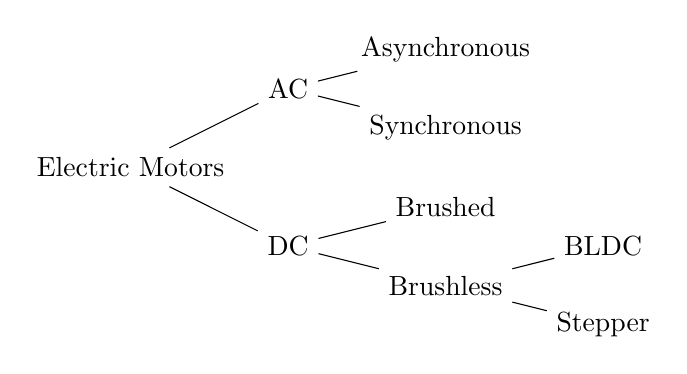
\begin{tikzpicture}[
        grow=right,
        level 1/.style={level distance=2cm, sibling distance=2cm},
        level 2/.style={level distance=2cm, sibling distance=1cm}
      ]
      \node {Electric Motors}
      child {
          node {DC}
          child {
              node {Brushless}
              child {
                  node {Stepper}
                }
              child {
                  node {BLDC}
                }
            }
          child {
              node {Brushed}
            }
        }
      child {
          node {AC}
          child {
              node {Synchronous}
            }
          child {
              node {Asynchronous}
            }
        };
    \end{tikzpicture}
  \end{center}
\end{frame}

\begin{frame}
  \frametitle{BLDC motors}

  \begin{figure}
    \centering
    \includegraphics[scale=0.3]{pmsm-outer.png}
    \caption{A BLDC (outer structure) from a floppy disk drive (Sebastian
      Koppehel, CC BY 3.0).}
  \end{figure}
\end{frame}

\begin{frame}
  \frametitle{BLDC motors}

  \begin{itemize}
    \item<1-> BLDC:\@ a \textbf{synchronous motor} using \textbf{direct current}
          (DC) power supply
    \item<2-> If back-EMF is sinusoidal: \textbf{PMSM} (Permanent Magnet
          Synchronous Motor)
    \item<3-> \textbf{High efficiency}, \textbf{high power-to-weight ratio},
          \textbf{high speed}\ldots
    \item<4-> The \textbf{rotor contains permanent magnets} that create a
          \textbf{constant magnetic field}
    \item<5-> Driven by an \textbf{inverter} controlled by a
          \textbf{microcontroller}
  \end{itemize}
\end{frame}

\begin{frame}
  \frametitle{BLDC motors}

  \begin{figure}
    \centering
    \includegraphics[scale=0.6]{pmsm.pdf}
    \caption{Schematic of a BLDC and its frames of reference.}
  \end{figure}
\end{frame}

\begin{frame}
  \frametitle{How does a BLDC motor spin?}

  \begin{itemize}
    \item<1-> Motor is driven by $\mathbf{120^{\circ}}$\textbf{-phased
            sinusoidal voltages}
    \item<2-> This results in a \textbf{rotating vector} in the abc frame
          constant in magnitude known as the \textbf{space-vector}
    \item<3-> \textbf{Currents} flowing through the windings will \textbf{induce
            a rotating magnetic field}
    \item<4-> The rotor \textbf{permanent magnet} will \textbf{rotate to keep
            aligned} with the generated field
  \end{itemize}

  \begin{figure}
    \centering
    \includegraphics[scale=0.25]{rotating-magnetic-field.pdf}
    \caption{Rotating magnetic field generated by sinusoidal phase currents
      (original: Svjo, CC-0).}
  \end{figure}
\end{frame}

\begin{frame}
  \frametitle{Field Oriented Control}

  \begin{itemize}
    \item<1-> Field Oriented Control (FOC) is a commonly used control technique
    \item<2-> Operates in the \textbf{dq space}, a \textbf{stationary frame}
          with respect to the rotor position (DC quantities!)
    \item<3-> Generated \textbf{torque is proportional} to the controlled
          variable $\mathbf{i_q}$
    \item<3-> Based on a set of \textbf{transformations} (Clarke and Park) and
          the knowledge of the \textbf{rotor position}, usually provided by a
          sensor
  \end{itemize}

  \begin{figure}
    \centering
    \includegraphics[scale=0.35]{cloop-full-schematic.pdf}
    \caption{Current (torque) control with Field Oriented Control (FOC).}
  \end{figure}
\end{frame}

% section: introduction --------------------------------------------------------

\section{Why Zephyr?}

\begin{frame}[plain]{}
  \begin{center}
    \Huge \textbf{Why Zephyr?}
  \end{center}
\end{frame}

\begin{frame}
  \frametitle{Before Zephyr\ldots why an RTOS?}

  \begin{itemize}
    \item<1-> Motor controllers can quickly become a \textbf{complex system}:
          \begin{itemize}
            \item Communications interface (MODBUS, CANopen\ldots)
            \item Additional peripherals (e.g.\ non-volatile memory,
                  sensors\ldots)
            \item Monitoring tasks
            \item \ldots and more!
          \end{itemize}
    \item<2-> \textbf{Hard to manage} everything in a bare-metal
          \textbf{\textit{super-loop} architecture}
    \item<3-> An \textbf{RTOS} provides a \textbf{scalable solution}:
          \begin{itemize}
            \item Allows \textbf{focusing on application development}
            \item Program \textbf{functions} are split into
                  \textbf{self-contained tasks}
            \item \textbf{Tasks are scheduled when needed}, improving program
                  flow and response time
            \item \textbf{Shared resources} are \textbf{easier to manage}
          \end{itemize}
  \end{itemize}
\end{frame}

\begin{frame}
  \frametitle{Why Zephyr?}

  \begin{itemize}
    \item<1-> Zephyr is \textbf{not only an RTOS}, it is an \textbf{ecosystem}
    \item<2-> \textbf{Modern build system} based on CMake
    \item<3-> Support for \textbf{Devicetree} and \textbf{Kconfig}
    \item<4-> \textbf{Vendor independent}, permissive license (Apache 2.0)
    \item<5-> \textbf{Best-in-class development practices}
    \item<6-> \textbf{Generic APIs} (e.g.\ serial, GPIO, I2C, SPI,
          sensors\ldots)
    \item<7-> \textbf{Built-in features} relevant for motor control:
          \begin{itemize}
            \item Direct access to vendor HALs
            \item Access to CMSIS packages, e.g.\ DSP
            \item Industrial field buses: CANopen, MODBUS
            \item Advanced debugging and tracing facilities
            \item \ldots and more!
          \end{itemize}
  \end{itemize}
\end{frame}

\begin{frame}[fragile]
  \frametitle{Devicetree}

  \begin{itemize}
    \item<1-> Devicetree: a hierarchical data structure that describes hardware
    \item<2-> \texttt{devicetree.h} API gives access to the information from the
          drivers or application
    \item<3-> A \textbf{versatile solution} compared to \textit{endless
            configuration headers}
  \end{itemize}

  \vspace{1em}

  \begin{codebox}[devicetree]
    &adc1 {
    currsmp: currsmp {
        compatible = "st,stm32-currsmp-shunt";
        pinctrl-0 = <&adc1_in1_pa0 &adc1_in7_pc1 &adc1_in6_pc0>;

        adc-channels = <1 7 6>;
        adc-trigger = <STM32_ADC_INJ_TRIG_TIM1_TRGO>;
      };
    };
  \end{codebox}

  \begin{center}
    \tiny
    \faLifeRing~\url{https://docs.zephyrproject.org/latest/guides/dts/intro.html}
  \end{center}
\end{frame}

\begin{frame}[fragile]
  \frametitle{Kconfig}

  \begin{itemize}
    \item<1-> Kconfig: a language to describe \textbf{software configuration
            options}
          \begin{itemize}
            \item Supports \textbf{multiple types} (bool, int\ldots)
            \item \textbf{Dependencies} can be specified
            \item Options can be \textbf{browsed and edited interactively}
          \end{itemize}
    \item<3-> Options \textbf{can be accessed} from both \textbf{C} code and the
          \textbf{build system}
  \end{itemize}

  \begin{codebox}[kconfig]
    config SPINNER_SVPWM_STM32
      bool "STM32 SV-PWM driver"
      default y if SOC_FAMILY_STM32
      select USE_STM32_LL_TIM
      select SPINNER_SVM
      select SPINNER_UTILS_STM32
      help
        Enable SV-PWM driver for STM32 SoCs
  \end{codebox}

  \begin{center}
    \tiny
    \faLifeRing~\url{https://docs.zephyrproject.org/latest/guides/kconfig/index.html}
  \end{center}
\end{frame}

\begin{frame}
  \frametitle{Kconfig}

  \begin{figure}
    \centering
    \includegraphics[scale=0.25]{kconfig.png}
    \caption{Interactive Kconfig browser.}
  \end{figure}
\end{frame}

% section: spinner -------------------------------------------------------------

\section{SPINNER}

\begin{frame}[plain]{}
  \begin{center}
    \includegraphics[scale=0.2]{spinner.pdf}
  \end{center}
\end{frame}

\begin{frame}
  \frametitle{What is SPINNER?}

  \begin{itemize}
    \item<1-> A proof-of-concept motor control firmware based on the
          \textbf{Field Oriented Control} principles
    \item<2-> Built on top of \textbf{Zephyr}
    \item<3-> Implements the \textbf{current (torque) control loop} using FPU
    \item<4-> Provides \textbf{driver interfaces} for:
          \begin{itemize}
            \item Feedback sensors, e.g. Halls
            \item SV-PWM
            \item Current sampling
          \end{itemize}
    \item<5-> Driver implementations for \textbf{STM32} (F3xx)
  \end{itemize}

  \begin{center}
    \faGithub~\url{https://github.com/teslabs/spinner}
  \end{center}
\end{frame}

\begin{frame}
  \frametitle{Supported boards}

  \begin{figure}
    \centering
    \includegraphics[scale=1]{p-nucleo-ihm002.jpg}
    \caption{P-NUCLEO-IHM002 (NUCLEO-F302R8 + X-NUCLEO-IHM07M1).}
  \end{figure}
\end{frame}

\begin{frame}
  \frametitle{SPINNER components}

  \begin{itemize}
    \item<1-> \textbf{SV-PWM}: Driver responsible for synthesizing space-vector
          using modulated (PWM) signals
    \item<2-> \textbf{Current sensing}: Driver responsible for sampling motor
          currents and calling current control loop
    \item<3-> \textbf{Feedback}: Driver responsible for sensing rotor position
    \item<4-> \textbf{Current control loop}: Component responsible for the motor
          currents regulation using FOC
  \end{itemize}

  \begin{figure}
    \centering
    \includegraphics[scale=0.35]{spinner-schematic.pdf}
    \caption{Block diagram of SPINNER core components.}
  \end{figure}
\end{frame}

\begin{frame}
  \frametitle{Design principles}

  \begin{itemize}
    \item<1-> Drivers provide a \textbf{generic interface}, allowing better
          \textbf{portability} and \textbf{testability}
    \item<2-> \textbf{Vendor HALs} (STM32 LL) are used: allows building on top
          of \textbf{battle-tested code}
    \item<3-> \textbf{Devicetree} is used to obtain all hardware description,
          including pinmux
    \item<4-> \textbf{Kconfig} is used to specify all software dependencies
    \item<5-> Firmware is \textbf{structured as a module}, following the Zephyr
          \texttt{example-application}
  \end{itemize}

  \vspace{1em}

  \begin{center}
    \scriptsize
    \faGlobeAmericas~\url{https://github.com/zephyrproject-rtos/example-application}
  \end{center}
\end{frame}

\begin{frame}
  \frametitle{Current sampling}

  \begin{itemize}
    \item<1-> Driver responsible for \textbf{sampling motor phase currents},
          usually by means of \textbf{shunt resistors}
    \item<2-> \textbf{Measurements} are \textbf{synchronized with SV-PWM}
    \item<3-> \textbf{Sampling rate} ranges \textbf{from 10 to 50 kHz}
    \item<4-> ADC \textbf{completion IRQ} calls the \textbf{current control
            loop}
    \item<5-> \textbf{Current control loop} needs to be run at a
          \textbf{predictable} rate
  \end{itemize}
\end{frame}

\begin{frame}[fragile]
  \frametitle{Current sampling: Zero Latency Interrupts}

  \begin{itemize}
    \item<1-> Zero Latency Interrupts (ZLI) execute at the
          \textbf{highest priority}
    \item<2-> \textbf{Not affected by interrupt locking}, i.e.
          \texttt{irq\_lock ()}
    \item<3-> Combined with Direct Interrupts results in
          \textbf{\textit{bare-metal} like performance}
    \item<4-> \textbf{Cannot interoperate} with the \textbf{Kernel}
    \item<5-> Only supported on Cortex-M if \texttt{CONFIG\_ZERO\_LATENCY\_IRQS}
          is enabled
  \end{itemize}

  \begin{codebox}[C]
    ISR_DIRECT_DECLARE(irq_routine)
    {
        ...
    }

    IRQ_DIRECT_CONNECT(irq, priority, irq_routine, IRQ_ZERO_LATENCY);
  \end{codebox}
\end{frame}

\begin{frame}
  \frametitle{Current sampling: Zero Latency Interrupts}

  \begin{figure}
    \centering
    \includegraphics[scale=0.19]{zli-cloop.png}
    \caption{Current sampling ADC JEOS interrupt configured as ZLI calling
      current control loop @ 30 kHz (P-NUCLEO-IHM002).}
  \end{figure}
\end{frame}

\begin{frame}
  \frametitle{Current sampling: Zero Latency Interrupts}

  \begin{figure}
    \centering
    \includegraphics[scale=0.19]{zli-disabled-cloop.png}
    \caption{Current sampling ADC JEOS interrupt \textbf{not} configured as ZLI
      calling current control loop @ 30 kHz (P-NUCLEO-IHM002).}
  \end{figure}
\end{frame}

\begin{frame}
  \frametitle{Current Loop}

  \begin{itemize}
    \item<1-> Current loop \textbf{controls motor currents} (and so
          \textbf{torque})
    \item<2-> Called after the completion of every current sampling
    \item<3-> Implements Field Oriented Control (FOC)
    \item<4-> The \textbf{most critical and resource demanding} control loop,
          \textbf{runs from 10 to 50 kHz}
  \end{itemize}

  \begin{figure}
    \centering
    \includegraphics[scale=0.4]{cloop-only-schematic.pdf}
    \caption{Current loop (highlighted blocks).}
  \end{figure}
\end{frame}

\begin{frame}
  \frametitle{Current Loop: CMSIS-DSP}

  \begin{itemize}
    \item<1-> CMSIS-DSP is a \textbf{suite of digital signal processing (DSP)
            functions} for use on Cortex-M and Cortex-A processors.
    \item<2-> Provides all \textbf{necessary functions} to implement the
          \textbf{current control loop}
    \item<3-> \textbf{Available on Zephyr} as a module!
    \item<4-> Used functionality can be enabled using
          \texttt{CONFIG\_CMSIS\_DSP\_*}
  \end{itemize}
\end{frame}

\begin{frame}[fragile]
  \frametitle{Current Loop: CMSIS-DSP}

  \begin{codebox}[C]
    /* compute sin and cos of electrical angle */
    arm_sin_cos_f32(eang, &sin_eang, &cos_eang);

    /* i_a, i_b -> i_alpha, i_beta */
    arm_clarke_f32(i_a, i_b, &i_alpha, &i_beta);
    /* i_alpha, i_beta -> i_q, i_d */
    arm_park_f32(i_alpha, i_beta, &i_d, &i_q, sin_eang, cos_eang);

    /* PI (i_d, i_q -> v_d, v_q) */
    v_d = arm_pid_f32(&pid_id, id_ref - i_d);
    v_q = arm_pid_f32(&pid_iq, iq_ref - i_q);

    /* v_d, v_q -> v_alpha, v_beta */
    arm_inv_park_f32(v_d, v_q, &v_alpha, &v_beta, sin_eang, cos_eang);
  \end{codebox}

  \begin{center}
    \tiny
    \faLifeRing~\url{https://arm-software.github.io/CMSIS_5/DSP/html/index.html}
  \end{center}
\end{frame}

\begin{frame}
  \frametitle{STM32 MCSDK 5.Y.1 comparison}

  \begin{itemize}
    \item<1-> MCSDK:\@ \textbf{official} STM32 motor control firmware
    \item<2-> Uses \textbf{fixed point arithmetic}
    \item<3-> Offers \textbf{more features} (sensorless, speed control, etc.)
  \end{itemize}

  \begin{figure}
    \centering
    \includegraphics[scale=0.14]{cloop-mcsdk-5y1.png}
    \caption{STM32 MCSDK 5.Y.1 current control loop @ 30 kHz (P-NUCLEO-IHM002).}
  \end{figure}
\end{frame}

% section: conclusions ---------------------------------------------------------

\section{Conclusions}

\begin{frame}[plain]{}
  \begin{center}
    \Huge
    \textbf{Conclusions}
  \end{center}
\end{frame}

\begin{frame}
  \frametitle{Conclusions}

  \begin{itemize}
    \item<1-> Zephyr allows \textbf{focusing on application development}
    \item<2-> Zephyr gives access to \textbf{powerful and modern tools}:
          Devicetree, Kconfig, CMake
    \item<3-> Zephyr comes with \textit{\textbf{batteries included}}, e.g.
          CMSIS-DSP
    \item<4-> Zephyr represents a \textbf{cultural-shift} on how development is
          done in the embedded industry
    \item<5-> \textbf{Zero Latency Interrupts (ZLI)} allow \textbf{bare-metal
            like performance}
    \item<6-> Access to \textbf{vendor HALs} is a \textbf{key feature} to speed
          up driver development
    \item<7-> Zephyr has a \textbf{great and supportive community}!
  \end{itemize}
\end{frame}

\begin{frame}[c]
  \begin{center}
    \huge
    \textbf{THANK YOU!} \\
    Questions? \\
    \vspace{2.5em}
    \normalsize
    \faFilePowerpoint~\url{https://github.com/teslabs/spinner-zds-2021} \\
    \vspace{1.5em}
    \faGithub~\url{https://github.com/teslabs/spinner} \\
    \faBook~\url{https://teslabs.github.io/spinner}
  \end{center}
\end{frame}

\end{document}
